\chapter{Methodology}\label{ch:methodology}

\section{Day-Ahead Forecasting Strategy}\label{sec:proposed-methods}

In DA nodal markets, energy prices are settled on an hourly basis, with 24 hours per market-day.
Participants are required to submit all trades --- a single trade consists of a \textit{location}, \textit{hour},
\textit{direction} (buy or sell), \textit{price}, and \textit{volume} --- for a given market-day no later than one-day
in advance.
Specifically, if the market-day is denoted by $T$, there is a trade-submission deadline on the day $T-1$ at which all
trades for $T$ are submitted.
For each node, prices must be forecasted for all 24 hours simultaneously.
Thus, for a set of $n$ price nodes a total of $n \times 24$ total price forecasts are required.
There is no consensus on the best forecasting methodology, with popular choices being
a single model creating a joint $n \times 24$ forecast~\cite{9520248, 9916722},
one model per-node with 24-hour joint forecasts~\cite{00000, 7744689, LAGO2018386},
one model with joint forecasts over the nodes independently per-hour~\cite{5741753, 7478156, 8733097},
and finally one model per-hour per-node\cite{en9080621}.

In this work, the DA price forecasting problem is approached using a single model to jointly forecast price densities
across all $n$ nodes and forecasts for each hour are generated independently.
This joint probabilistic forecasting strategy captures the complex non-linear price distribution between nodes for each
hour given fundamental market forecasts.
That is, if $\mathcal{X}_t \subseteq \mathbb{R}^n$ is a random variable with realizations $x_t$ of the nodal LMPs for a
specific market-hour $t$ and $c_t \in \mathbb{R}^m$ is a real-valued vector of fundamental market forecasts for the
same market-hour, we propose a model which characterizes the joint conditional probability distribution
 $p_{\mathcal{X}_t}(x_t | c_t)$.
Thus when forecasting an entire market-day, 24 independent probability densities are characterized for each hour as
shown in Figure~\ref{fig:da_fc_task}.

\begin{figure}[htbp]
    \caption[Proposed forecasting methodology in relation to the day-ahead forecasting timeline]{
        Proposed day-ahead forecasting methodology.
        At the time of the trade submission deadline 24 joint conditional
        distributions have been characterized for each hour of the upcoming market-day.
    }
    \begin{center}
        \setlength{\fboxsep}{0pt}%
        \setlength{\fboxrule}{1pt}%
%        \fbox{
            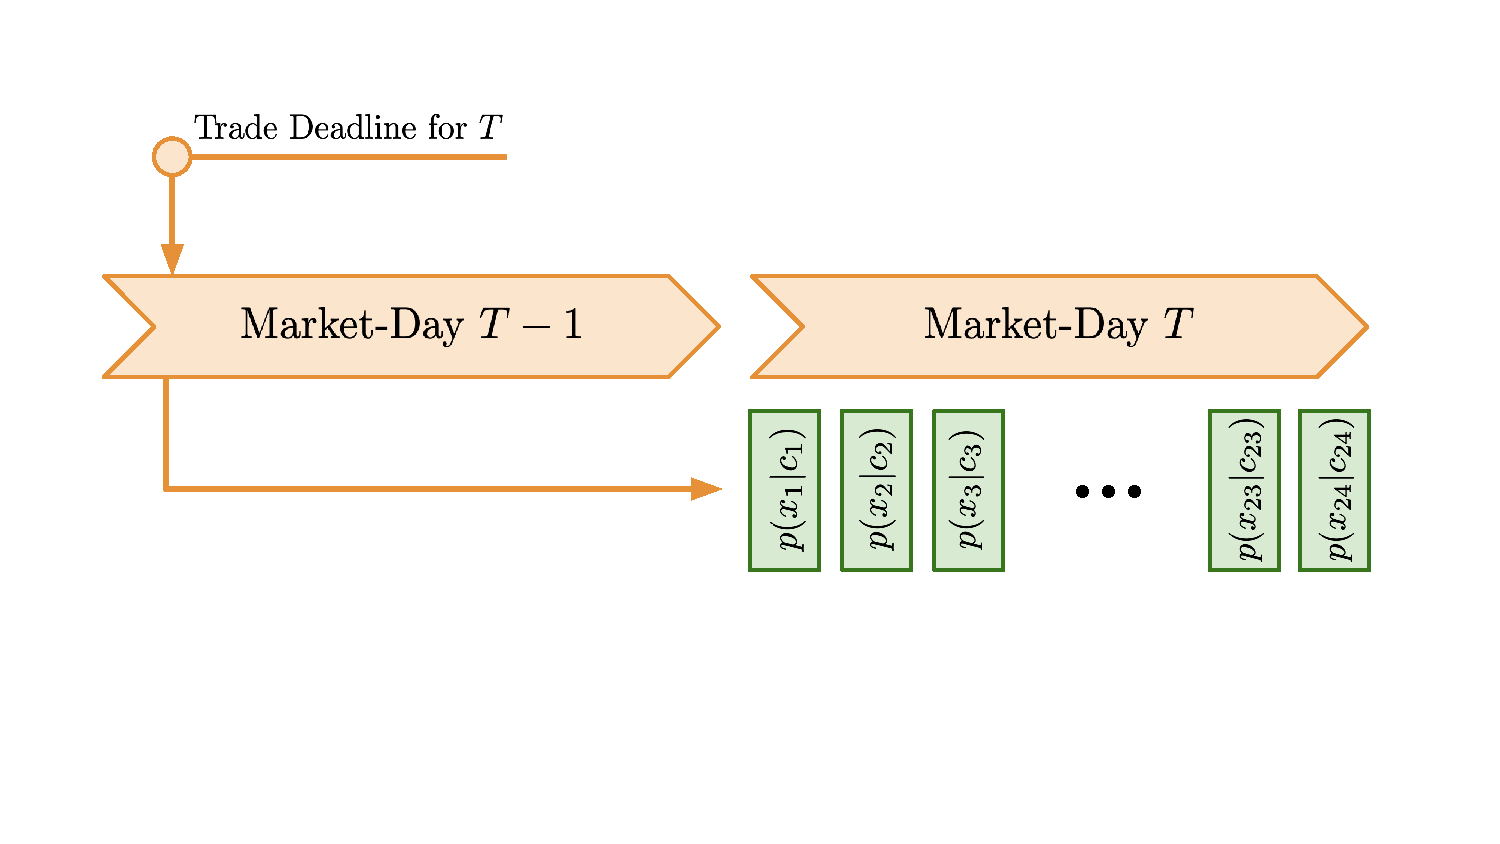
\includegraphics[width=120mm]{figs/da_fc_task.pdf}
%        }
    \end{center}
    \label{fig:da_fc_task}
\end{figure}

The proposed strategy to characterize the joint conditional density estimators is as follows,

\begin{enumerate}
    \item Select a set of $n$ price nodes for which to generate forecasts and a set of $m$ quantities
    that affect day-ahead nodal energy prices and are available before the trade submission deadline.

    \item Choose an $n$-dimensional probability distribution to be the reference distribution $\eta$.
    Typical choices are standard uniform or Gaussian distributions, however any distribution with tractable
    log-likelihood evaluations and sampling capabilities could be used.

    \item Construct a diffeomorphism $f_\theta : \mathbb{R}^n \mapsto \mathbb{R}^n$ characterized by the cINN architecture
    described in Section~\ref{sec:conditional-invertible-neural-network}.
    Additionally we must choose a suitable feature extraction network $h(c_t)$.
    Omission of the feature extraction network is equivalent to $h(c_t) = \mathbf{I}c_t$ where $\mathbf{I}$
    is the $m \times m$ identity matrix.
    Note that the feature extraction network and its respective parameters are included when referring to $f_\theta$.

    \item Construct a discriminator $D_\phi : \mathbb{R}^{n + m} \mapsto [0,\;1]$ with which to evaluate $\mathcal{L}_{\text{ADV}}$,
    and select a value for $\lambda_{\text{ADV}}$ to control the emphasis on $\mathcal{L}_{\text{MLE}}$ or
    $\mathcal{L}_{\text{ADV}}$ in the hybrid loss function.

    \item Update the parameters of $f_\theta$ and $D_\phi$ using the Adam stochastic gradient descent algorithm~\cite{adam_optim}.
    Mini-batches of pairs from the set of $N$ historical training observations
    $\left\{ \left( x_i,\; c_i \right) \right\}_{i=1}^N$ are used to evaluate $\mathcal{L}_{\text{MLE}}$.
    Samples $\left\{ z_i \right\}_{i=1}^N \sim \eta$ are drawn and the conditional push forward operation is applied
    to form synthetic price samples $\hat{x_i} = f_\theta(z_i; c_i)$.
    Mini-batches of pairs from the resulting set $\left\{ \left(\hat{x_i},\; c_i \right) \right\}_{i=1}^N$ are used to
    evaluate $\mathcal{L}_{\text{ADV}}$.
    Note the conditional quantities are identical in both the real and synthetic mini-batches.
\end{enumerate}

\section{Datasets}\label{sec:datasets}

\begin{itemize}
    \item \textbf{Prices}: Historical day-ahead LMP timeseries are obtained for 45 price nodes in the PJM market
    capturing prices in all 25 load zones and the interconnections with neighboring markets.
    These prices are published by PJM on an hourly basis shortly after the trade submission deadline for the upcoming
    market-day has passed.
    The full list of nodes can be found in Appendix~\ref{ch:list-of-pjm-price-nodes}.

    \item \textbf{Load Forecasts}: Historical hourly load forecasts are obtained for each of the 25 load zones in PJM\@.
    Zonal load forecasts represent the expected energy demand in mega-watts (MW) in each sub-region of PJM for a given
    market-hour and are published on an hourly basis by PJM\@.
    These forecasts are available for participants to use during trade generation and submission.
    The full list of load zones can be found in Appendix~\ref{ch:list-of-pjm-load-zones}.

    \item \textbf{Wind Generation Forecasts}: A historical hourly timeseries is obtained for the ISO level wind generation
    near-term forecast.
    This forecast is published by PJM and represents the expected total generation (MW) from all wind turbine renewable
    power plants in PJM for a given market-hour and is available to participants during trade generation and submission.

    \item \textbf{Meteorological Forecasts}: Historical hourly meteorological forecasts are obtained for a collection
    of NOAA weather stations in and around PJM\@.
    There are a total of 52 weather stations spanning the entire geographical region of PJM\@.
    Each weather station reports expected hourly wind speeds (mph), temperature (°F), and dew-point (°F).
    These forecasts are available to participants during trade generation and submission.
    The full list of NOAA weather stations can be found in Appendix~\ref{ch:list-of-noaa-weather-stations}.

    \item \textbf{Natural Gas Prices}: Historical natural gas spot price timeseries are obtained for the TETCO-M3 hub.
    The prices reflect the daily volume-weighted-average-price (VWAP) and are reported on a daily basis.
    The daily VWAP for the upcoming market-day is unknown, so instead the most recent daily VWAP at the time of
    trade-generation is persisted and used for all 24 hours in the price forecast.
\end{itemize}

Timeseries for all of the above datasets are captured for the entirety of years 2019, 2020, and 2021.

\section{Data Pre-Processing}\label{sec:data-pre-processing}

To improve the numerical stability of the stochastic gradient descent algorithm we preprocess all
aforementioned quantities to normalize the disparate scaling between feature classes.
A standard linear scaling strategy on a per-quantity basis was found to be sufficient when applied to all quantities
despite more complex variance stabilizing scaling strategies proposed in energy forecasting literature~\cite{7997921}.
Let $\left\{ y_i \right\}_{i=1}^N$ be a historical timeseries for a scalar quantity such that the first $k < N$ values
are used for model training and the remaining values are held out for validation, then the transformation
$\bar{y}_i = \frac{y_i - \hat{\mu}_y}{\hat{\sigma}_y}$ is applied for $1 \leq i \leq N$ where
$\hat{\mu}_y,\;\hat{\sigma}_y$ are the empirical mean and standard deviation of training set for the respective quantity.

In addition to the scaled fundamental market forecasts, temporal encodings of the upcoming market-time $t$ are constructed.
Assuming $t$ contains information on the hour-of-day and elapsed-days-since-epoch (1-1-1970), given by
$\text{hour}(t) \in \{1, 2, \dots, 24\}$ and $\text{day}(t) \in \mathbb{N}$ respectively, we construct the following three
sinusoidal encodings to relate temporally-similar market-times,

\begin{align*}
    \text{Hour-of-Day} &= \left[ \cos\left( \text{hour}(t) \times \frac{2\pi}{24} \right), \; \sin\left( \text{hour}(t) \times \frac{2\pi}{24} \right)\right] \\
    \text{Day-of-Week} &= \left[ \cos\left( \text{day}(t) \times \frac{2\pi}{7} \right), \; \sin\left( \text{day}(t) \times \frac{2\pi}{7} \right)\right] \\
    \text{Day-of-Year} &= \left[ \cos\left( \text{day}(t) \times \frac{2\pi}{365} \right), \; \sin\left( \text{day}(t) \times \frac{2\pi}{365} \right)\right]
\end{align*}


Note that we are targeting forecasts on 45 price nodes, thus the reference and target
distributions are 45-dimensional, however, the affine coupling block architecture requires an even number of
dimensions for the component partitions to be of equal sizes.
To remedy this, a dummy dimension is created by appending zeros to the price-vector observations bringing the number of
dimensions up to 46.
When sampling price forecasts, values from dummy dimension are dropped after applying the push-forward operation.

\section{Baselines}\label{sec:baselines}

To validate the results of our proposed forecasting methodology we compare against the following three point-forecast
baselines.
Note that the first two baselines come from the open-source \texttt{epf-toolbox}~\cite{epftoolbox} python library,
however, the models provided in this toolbox are meant to be trained on the datasets provided by this toolbox.
The dataset available for PJM only includes day-ahead prices for three price nodes and load forecasts for a single
load zone and the total system-wide load.
As such, the models are modified to use all available exogenous quantities and the
proposed data pre-processing methodologies, however, the proposed sinusoidal temporal encoding are omitted in favor of
the temporal encodings originally defined in the \texttt{epf-toolbox}.

\subsection{LASSO Estimated Auto-Regressive}\label{subsec:lasso-estimated-auto-regressive}

The \textit{LASSO estimated auto-regressive model} is a parameter-rich auto-regressive model with the capacity to handle
exogenous variables.
Let $d(t)$ and $h(t)$ be shorthand for the functions $\text{day}(t),\; \text{hour}(t)$ respectively for a market-time
$t$, $p_{d(t)} \in \mathbb{R}^{24}$ be the realized day-ahead price at a single price node at market-times on the same
day as $d(t)$, $x^j_{d(t)} \in \mathbb{R}^{24}$ be the $j^{\text{th}}$ exogenous quantity at market-times on the same market-day
as $d(t)$, and $\textbf{e}_{j}$ the $j^{\text{th}}$ column of the $7\times7$ identity matrix.
Then the forecast $\hat{p}_t$ for an upcoming market-time $t$ at a single node is defined as,

\begin{align*}
    \hat{p}_t(\theta) = & \; \sum_{k \in \left\{ 1, 2, 3, 7 \right\}} {\theta^0_{\left[ 24 \times (k-1) : 24 \times k \right]}}^\mathsf{T} p_{d(t) - k} \\
                        & +  \sum_{j=1}^m {\theta^j_{\left[0:24\right]}}^\mathsf{T} x^j_{d(t)} + {\theta^j_{\left[24:48\right]}}^\mathsf{T} x^j_{d(t) - 1} + {\theta^j_{\left[48:96\right]}}^\mathsf{T} x^j_{d(t) - 7} \\
                        & +  {\theta^{m + 1}}^\mathsf{T} \textbf{e}_{\left[d(t) \mod 7\right]} \\
                        & +  \epsilon.
\end{align*}


Where $\theta^k \in \mathbb{R}^r$ are parameters with transpose $\theta^\mathsf{T} \in \mathbb{R}^{1 \times r}$ and
parameters ${\theta^k_{\left[i:j\right]}}$ are a subset of parameters $\theta^k$
characterized by the entries spanning the interval $[i, j)$ with $0 < i < j \leq r$, and
$\theta^\mathsf{T} = [{\theta^0}^\mathsf{T} \dots {\theta^{m+1}}^\mathsf{T}]$ is the full set of parameters for the LEAR model.
In this definition, $\theta^0$ are auto-regressive parameters, $\theta^{1} \dots \theta^{m}$ are parameters
for exogenous variables, and $\theta^{m+1}$ are parameters for a day-of-the-week temporal one-hot encoding. $\epsilon$
is a standard error term.

The LEAR model is trained using sum-of-squares loss between the forecasted price $\hat{p}_t$ and the realized price
$p_t$ applying a $\ell_1$ weight penalty with intensity $\lambda \geq 0$ on parameters $\theta$ to encourage sparsity.
Note, $\theta$ is optimized only for a single hour, thus when training only observations at a specific hour are considered.
Over a set of $N$ training days, $\theta_h$ is optimized for a specific market hour $h$ as,

\begin{equation}
    \min_{\theta_h} \sum_{d=1}^N \left(\hat{p}_{t=(d, h)}(\theta_h) - p_{t=(d, h)}\right)^2 + \lambda \lVert \theta_h \rVert_1. \nonumber
    \label{eq:lear_loss}
\end{equation}

\subsection{Deep Neural Network}\label{subsec:deep-neural-network}

The \textit{deep neural network} (DNN) model is a simple feed-forward neural network which produces point forecasts for
a single node at all 24 market-hours simultaneously.
The DNN is trained on the same quantities as the LEAR model, that is for the upcoming market-day $d$, the neural network
forecasts the price vector $\hat{p}_d$ using price history $\left\{ p_{d-1}, p_{d-2}, p_{d-3}, p_{d-7} \right\}$,
exogenous forecasts and history $\left\{ x^j_{d}, x^j_{d - 1}, x^j_{d-7} \right\}$ for exogenous quantities
$1 \leq j \leq m$, and temporal encoding $\mathbf{e}_{\left[d \mod 7\right]}$.
The DNN is trained using root-mean-squared (RMS) loss, and a full description of hyperparameters can be found in
Appendix~\ref{ch:model-and-optimizer-hyperparameters}.

\subsection{Commercial Optimal Powerflow Solver}\label{subsec:commercial-optimal-powerflow-solver}

The commercial optimal powerflow solver (OPF) is a tool that produces joint point LMP forecasts over a set of nodes
for a single hour by solving a variation of the \textit{security constrained economic dispatch} (SCED) optimization problem.
The process by which LMPs are actually produced is derived from a solution of this problem, and the OPF tool
aims to forecast the parameters of the SCED problem such that its solution yields price forecasts.
Explanation of SCED and related power system optimization problems are beyond the scope of this work, however a review
of these problems and the tools used to solve them can be found in~\cite{opf_textbook}.
Forecasts from commercial OPF tools are often highly desirable for their accuracy and because they are derived from the
true physical properties underpinning grid and market behavior.

\section{Evaluation Metrics}\label{sec:evaluation-metrics}

Root-mean-squared-error (RMSE), mean-absolute-percentage-error (MAPE) and mean-absolute-error (MAE) are common metrics
in energy price forecasting literature, however, they are only valid for use with point forecasts.
Of those metrics, MAE is the best metric for energy price forecasts because the linear errors best
represent the actual losses one would incur when trading --- that is the profit or loss incurred on a trade scales
linearly with the difference between the buy and sell prices, analogous to the absolute error between realized and
forecasted prices.
Using these metrics for our forecasts would require distillation of the information-rich probabilistic forecasts
down into point forecasts.
Instead, we use the \textit{continuous ranked probability score} (CRPS)~\cite{crps_rules}, which generalizes the absolute error
metric to probabilistic forecasts.
Let $\mathbbm{1}_{\left[x \in A\right]}$ be an indicator which takes the value $1$ when $x \in A$ and $0$ otherwise.
For a univariate random variable $\mathcal{X} \subseteq \mathbb{R}$ with the probabilistic forecast represented by the
cumulative density function $F_\mathcal{X}$, the CRPS of $F_\mathcal{X}$ against a realization $y \in \mathbb{R}$ is defined
as

\begin{equation}
    \text{CRPS}_{F_\mathcal{X}}(y) = \int_{-\infty}^{\infty} \left(F_\mathcal{X}(u) - \mathbbm{1}_{\left[ y \leq u \right]}\right)^2 du.
    \label{eq:crps_int}
\end{equation}

We may interpret~\eqref{eq:crps_int} as the mean squared error between the forecast c.d.f. and the c.d.f. given by a
Dirac delta function at the realized value.
The CRPS generalizes of the absolute error of a point forecast, illustrated by the substitution of
$\mathbbm{1}_{\left[ x \leq u\right]}$ for $F_\mathcal{X}(u)$ given a point forecast $x$,

\begin{equation*}
    \int_{-\infty}^{\infty} \left(\mathbbm{1}_{\left[ x \leq u\right]} - \mathbbm{1}_{\left[ y \leq u \right]}\right)^2 du =
    \int_{\min(x, y)}^{\max(x, y)} du = |x - y|,
\end{equation*}
thus enabling direct comparison of probabilistic and point forecasting methods.

In practice, we do not have access to the marginal c.d.f.s of each price node.
Instead, we draw a set of $M$ samples from our joint conditional density estimator and compute the empirical marginal
c.d.f of the $j^{\text{th}}$ price node, $\hat{F}_{\mathcal{X}^j}$, as

\begin{equation}
    \hat{F}_{\mathcal{X}^j}(u) = \frac{1}{M} \sum_{i=1}^M \mathbbm{1}_{\left[ x_i^j \leq u \right]}
    \label{eq:emp_cdf}.
\end{equation}
From which we estimate the CRPS on the $j^{\text{th}}$ price node, $\widehat{\text{CRPS}}_{\hat{F}_\mathcal{X}^j}$, by
the substitution of~\eqref{eq:emp_cdf} into~\eqref{eq:crps_int}\footnotemark.

\footnotetext{Note that this form of the CRPS estimator is a biased estimator. For a description of an un-biased
counterpart and comparisons between various estimators refer to~\cite{crps_unbiased}.
For the remainder of this paper we continue to reference the estimator characterized by the substitution of
~\eqref{eq:emp_cdf} into~\eqref{eq:crps_int} as we believe the relevant behavior of the estimator is clearest in this
form.}

As this CRPS metric is only defined for univariate distributions, univariate forecasts for each price node are obtained
by marginalizing samples drawn from the entire joint distribution.
The average CRPS score over all price nodes for a single hour $t$, denoted here as mCRPS, is taken as a
single distilled metric directly comparable to the MAE of a point forecast at hour $t$ averaged over the price nodes.

\begin{equation}
    \widehat{\text{mCRPS}}_{\mathcal{X}_t}(y) = \frac{1}{n} \sum_{j=1}^n \widehat{\text{CRPS}}_{\hat{F}_{\mathcal{X}^j_t}}(y^j)
    \label{eq:mcrps}
\end{equation}

Additionally, the median and $99\%$-ile \textit{negative log-likelihood} (NLL) metrics are evaluated on the validation dataset.
A natural question is why use the median and $99\%$-ile NLL scores when the typical metric is the mean NLL
(equivalent to $\mathcal{L}_{\text{MLE}}$).
We found that despite being a valuable metric for training and parameter updates, tracking and evaluating mean NLL was
unstable on our dataset due to outlier sensitivity.
We would often experience a small set, or even a single validation example, that would have incredibly large NLL
values causing the mean calculations to be biased by the outliers leading to unstable results making fair model comparisons
difficult.
Tracking median NLL values was found to be better for model comparisons as the metric is robust to outlier examples.
The inclusion of the $99\%$-ile NLL proves useful as a large $99\%$-ile error imply
the model is poorly fit beyond a handful of outlier observations.
While certain regularization techniques we found to help reduce this behavior, we still consider it an open problem for
future research to analyze model sensitivity and determine methods to improve robustness against these outlier evaluations.
